\documentclass[12pt]{article}
 
\usepackage[noend]{algpseudocode}
\usepackage{algorithm}
\usepackage{algorithmicx}
\usepackage{float}
\usepackage{graphicx}
\usepackage[margin=0.75in]{geometry} 
\usepackage{amsmath,amsthm,amssymb}
\usepackage{dsfont}
\usepackage{subcaption}
\usepackage{amsthm}
\usepackage{mathtools,amssymb}
\usepackage{wrapfig}
\usepackage{hyperref}
\usepackage[font=small,skip=-20pt]{caption}
\allowdisplaybreaks

\newtheorem*{definition}{Definition}
\newtheorem*{question}{Question}
\newtheorem{theorem}{Theorem}
\newtheorem{proposition}[theorem]{Proposition}
\newtheorem{claim}[theorem]{Claim}
\newtheorem{lemma}[theorem]{Lemma}
\newtheorem{corollary}[theorem]{Corollary}
\newtheorem{conjecture}[theorem]{Conjecture}
 
\newcommand{\N}{\mathbb{N}}
\newcommand{\Z}{\mathbb{Z}}
\newcommand{\R}{\mathbb{R}}
\newcommand{\Rgz}{\mathbb{R}_{\ge 0}}

\newcommand{\ip}[2]{\left\langle{#1},{#2}\right\rangle}
\newcommand{\norm}[1]{\left\lVert{#1}\right\rVert}
\newcommand{\sizeof}[1]{\left\lvert{#1}\right\rvert}

\newcommand{\woloss}{without loss of generality }

\DeclareMathOperator*{\argmin}{arg\,min}
\DeclareMathOperator*{\argmax}{arg\,max}
\DeclareMathOperator*{\cone}{cone}
\DeclareMathOperator*{\hull}{hull}

\newcommand{\1}[1]{\mathds{1}[{#1}]}
\renewcommand{\P}[1]{\mathds{P}\left[{#1}\right]}
\newcommand{\E}[1]{\mathds{E}\left[{#1}\right]}
\newcommand{\Var}[1]{\mathrm{Var}[{#1}]}

\newcommand{\unit}{\mathds{1}}

% \renewcommand{\thesubsection}{\thesection.\alph{subsection}}
% \renewcommand\thesubsection{\ \ (\alph{subsection})}


\begin{document}

\begin{claim} \label{clm:pair}
For any pair of points $i = (i_1, i_2), j = (j_1, j_2) \in X$, where neither dominates the other, let $a = (a_1, a_2) \in \R_{\geq 0}^2$ be the preference weight vector that gives $i =_a j$, then for any preference weight vector $b = (b_1, b_2) \in \R_{\geq 0}^2$,
\begin{enumerate}
	\item \label{clm:pair1} $\frac{a \times b}{\norm{a \times b}} > 0$ if and only if $i >_b j$.
	\item \label{clm:pair2} $\frac{a \times b}{\norm{a \times b}} < 0$ if and only if $i <_b j$.
\end{enumerate}
\end{claim}

\begin{figure}
    \centering
    \begin{subfigure}[b]{0.25\textwidth}
        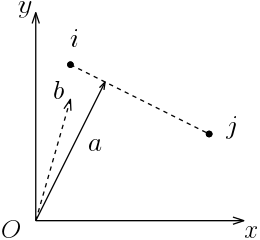
\includegraphics[width=\textwidth]{clm1}
        \caption{Claim}
        \label{fig:clm1}
    \end{subfigure}
    ~ %add desired spacing between images, e. g. ~, \quad, \qquad, \hfill etc. 
      %(or a blank line to force the subfigure onto a new line)
    \begin{subfigure}[b]{0.25\textwidth}
        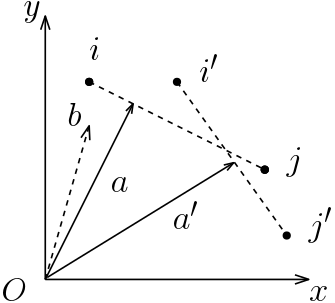
\includegraphics[width=\textwidth]{lemma1}
        \caption{Lemma}
        \label{fig:lemma1}
    \end{subfigure}
    \vspace{20pt}
    \caption{Illustrations}
\end{figure}

\begin{proof}
\ref{clm:pair1} and \ref{clm:pair2} are completely analogous, here we only prove \ref{clm:pair1}.
\begin{itemize}
	\item ``$\implies$'':
	On the one hand, from $\frac{a \times b}{\norm{a \times b}} > 0$ we have
	\begin{equation} \label{eqn:crossprod}
		a_1 b_2 - a_2 b_1 < 0 \implies a_1 < \frac{b_1}{b_2} a_2.
	\end{equation}
	On the other hand, by $i =_a j$,
	\begin{equation} \label{eqn:dotprod}
		a_1 i_1 + a_2 i_2 = a_1 j_1 + a_2 j_2 
		\implies a_1 (i_1 - j_1) = a_2 (j_2 - i_2).
	\end{equation}
	Plug (\ref{eqn:crossprod}) into (\ref{eqn:dotprod}), $a_2 (j_2 - i_2) < \frac{b_1}{b_2} a_2 (i_1 - j_1)$, this gives
	\[
		b_1 i_1 + b_2 i_2 > b_1 j_1 + b_2 j_2
		\implies i >_b j.
	\]

	\item ``$\impliedby$'':
	From (\ref{eqn:dotprod}) we get
	\begin{equation} \label{eqn:dotprod2}
		\frac{j_2 - i_2}{i_1 - j_1} = \frac{a_1}{a_2}.
	\end{equation}
	By $i >_b j$ and (\ref{eqn:dotprod2}),
	\[
		b_1 i_1 + b_2 i_2 > b_1 j_1 + b_2 j_2
		\implies \frac{b_1}{b_2} > \frac{j_2 - i_2}{i_1 - j_1} = \frac{a_1}{a_2}
		\implies a_1 b_2 - a_2 b_1 < 0
		\implies \frac{a \times b}{\norm{a \times b}} > 0.
	\]
\end{itemize}
\end{proof}

Using Claim \ref{clm:pair} we are able to show the following lemma.

\begin{lemma} \label{lem:pair}
Let $i, j, i', j'$ be two pairs of points in $X$ satisfying
\begin{itemize}
	\item neither of $i, j$ dominates the other: $i_1 < j_1$ and $i_2 > j_2$,
	
	\item neither of $i', j'$ dominates the other: $i_1' < j_1'$ and $i_2' > j_2'$,
	
	\item the slope of line $ij$ is less than the slope of line $i'j'$: $\frac{j_2 - i_2}{j_1 - i_1} < \frac{j_2' - i_2'}{j_1' - i_1'}$.
\end{itemize}
Then for any preference weight vector $b \in \mathbb{R}_{\geq 0}^2$,
\begin{enumerate}
	\item \label{lem:pair1}
	If $i >_b j$, $i' >_b j'$.
	
	\item \label{lem:pair2}
	If $j' >_b i'$, $j >_b i$.
\end{enumerate}
\end{lemma}

\begin{proof}
Again \ref{lem:pair1} and \ref{lem:pair2} are symmetric, we only prove \ref{lem:pair1}.
Let $a, a'$ be the preference weight vectors that gives $i =_a j$ and $i' =_{a'} j'$ respectively.
By definition of $a'$,
\begin{equation} \label{eqn:aprime}
	a_1' i_1' + a_2' i_2' = a_1' j_1' + a_2' j_2'
	\implies \frac{a_1'}{a_2'} = \frac{j_2' - i_2'}{i_1' - j_1'}.
\end{equation}
Since $i >_b j$,
\begin{equation} \label{eqn:ij}
	b_1 i_1 + b_2 i_2 > b_1 j_1 + b_2 j_2
	\implies \frac{b_1}{b_2} > \frac{j_2 - i_2}{i_1 - j_1}.
\end{equation}
From the relation of slopes we have
\begin{equation} \label{eqn:slope}
	\frac{j_2 - i_2}{i_1 - j_1} > \frac{j_2' - i_2'}{i_1' - j_1'}.
\end{equation}
Combine (\ref{eqn:aprime})(\ref{eqn:ij})(\ref{eqn:slope}) we get
\[
	 \frac{b_1}{b_2} > \frac{j_2 - i_2}{i_1 - j_1} > \frac{j_2' - i_2'}{i_1' - j_1'} = \frac{a_1'}{a_2'}
	 \implies a_1' b_2 - a_2' b_1 < 0 
	 \implies \frac{a' \times b}{\norm{a' \times b}} > 0.
\]
By Proposition \ref{prop:pair}, this implies $i' >_b j'$.
\end{proof}

Let $P_2$ be a set of $2$-dimensional preferences on $[n]$.

\begin{theorem} \label{thm:p2}
$\sizeof{P_2} \leq \binom{n}{2} + 1.$
\end{theorem}

\begin{proof}
We prove this upper bound algorithmically.
Consider the following algorithm of generating a preference in $P_2$ given $X$:

\begin{algorithm} \label{alg:PreGenP2}
\begin{algorithmic}[1]
	\State Relabel all points in $X$ such that $y_1 \geq y_2 \geq \cdots \geq y_n$
	\ForAll {$i, j \in X, i < j$}
		\State Compute slope $s_{ij}$
		\If {$s_{ij} < 0$}
			\State $L \gets s_{ij}$ \Comment{Suppose that $L[1]$ is the first element in the list $L$}
		\EndIf
	\EndFor
	\State Sort $L$ in ascending order
	\State Choose a pivot $p \in \{0, \dots, \sizeof{L} \}$
	\If {$p \geq 1$}
		\State Let $L[p] = s_{ij}$, set $i >_a j$
	\EndIf
	\If {$p+1 \leq \sizeof{L}$}
		\State Let $L[p+1] = s_{i'j'}$, set $i' <_a j'$
	\EndIf
	\State Output $>_a$
\end{algorithmic}
\caption{Preference Generator for $P_2$}
\end{algorithm}

\begin{wrapfigure}{r}{0.2\textwidth}
  \begin{center}
    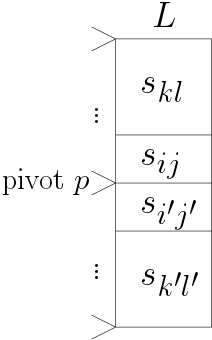
\includegraphics[width=0.18\textwidth]{thmp2}
  \end{center}
  \vspace{20pt}
  \caption{List $L$}
\end{wrapfigure}

Lemma \ref{lem:pair} ensures that by setting $i <_a j$ and $i' >_a j'$ in steps 8-11, all pairs $k,l$ before $i,j$ in list $L$ are set to $k <_a l$, and all pairs $k', l'$ after $i', j'$ in $L$ are set to $k' <_a l'$.
Moreover, there is a one-to-one correspondence between the actual preference, and choosing a pivot to flip from $<_a$ to $>_a$.
Since $\sizeof{L} \leq \binom{n}{2}$, and the number of pivots that we can choose from is $\sizeof{L} + 1$, we get that $\sizeof{P_2} \leq \binom{n}{2} + 1$.

The upper bound is tight.
ADD the example here!
\end{proof}
\end{document}